\section{Method}

The practicum was divided into three subareas, focusing on disection of the model and extrapolating the summary that would be used to robustly identify the internal structure of the model to enable the model synopsis to be stored in in a repository. The second section was to generate a unique signature for the model that is verified with minor and major changes to both the weights and biases, but also to quickly identify the model structure. The third part was discoving the best method to store they model summaries, so that they can be reused, pulled back and compared with the model currently in development, training or deployment.

The final method investigated in the practicum was application. On top of the original aim of determining the evolutionary tree of the model, other applications such as identifying difference between models that are in the process of being trained, as well as identifying portions of the training or deployment that would assist other methods of observability for model development, trust determination and internal visualisation.

\subsection{Developing a Robust Model Synopsis}
The first part of the delivery required that a model, in this case a CNN model in Keras, could be reduced to an information block that each layer contains a summary of the layer that can record any changes in the weights and biases. The structure of a model consists of a number of standard information points that are consistent across all deep learning processes. While we initially focused on CNNs, it became clear that any model could be used. A model consists of:

\begin{enumerate}
\item An Input Shape. In the case of vision applications, this consists of an image with width, height and colour depth, which is usually three.
\item Dense Application Layers, such as Pooling, Convolution or reduction layers which can contain a heavily connected series of filters, activation functions and weight and bias metrics.
\item Output layers. One or a number of prediction or output layers. In transfer learning, the output layers can change based on the prediction expanding or contracting.
\end{enumerate}

To be able to break down the model, it is nevessary to examing the layers. Within each of the layers, there are is a series of sublayers that. In all cases, these are in the form of series of tuples that have a single or multi-dimensional series of weights, plus a set of biases. Theoretically, these values can contain any number, while on inspection, the majority are within the bounds of a number series that can be tuned up or down in very small increments. it is within these layers that we will extract the layer identification information. 

For the benefit of breaking down a full layer across all dimensions, we examined a number of mathmatical options to identify the data underneath. It was important at this stage to focus on the minimal amount of information that would enable a unique signature to be generated. Experiments were completed to give an indication of distribution of data, which would assist in visualising the direction of training, in the form of layer-wide histograms or each dimension, and producing a \textit{histogram of gradients}-style overview. These were reduced in favour of two elements - Standard Deviation and Skew.

Skew:
\[ G_1=\frac{k_3}{k_2^{3/2}}=\frac{\sqrt{N(N-1)}}{N-2}\frac{m_3}{m_2^{3/2}}. \]

Standard Deviation of N Numbers
\[ \frac1N\sum_{i=1}^n\left(x^i-\overline x\right)^2 \]

Of all the averaging functions avaiable, the implementation of Standard Deviation in the python numpy library was able to reduce every single element to a single 64bit float. A second indication for skew was used to identify the drift of the standard deviation direction, and is included to ensure that movement of elements that retain the same Standard Deviation will not break the soltion.

\subsection{Generating a Unique signature}
Once we had every layer reduced to a number of identification values, we aggregated these together and together with a breakdown of the structure, a signature was generated. 

\begin{table}[h]
    \caption{Values generated from evaluated model}
    \setlength\tabcolsep{0pt} % make LaTeX figure out intercolumn spacing
    \begin{tabular}{@{} |p{2cm}|p{6.5cm}| @{}}
        Mean    & The average value of all layers across all dimension \\ \hline 
        StdDev  & An indication of the deviation of values, to assist in seeing how the values are weighted \\ \hline
        Histogram & A Histogram of the distribution of values across the layer. This will assist in giving a more informed distribution. As there are a large number of potential entries in the dense layers, from binary to minute changes in float values, the Histogram will be split between the values smallest non-zero granularity and the largest value across 10 bins. \\ \hline
        Name.   & Name of Layer \\ \hline
        Angle of Data & This is a single value representing the weighting of a Hash of the Layer Values (weights and biases) \\ 
    \end{tabular}
\end{table}

\subsection{Robustly Recording Changes}
As we now have a method of identifying the model in a broken down format, the next stage is to record and apply a signature to the model. There are a number of methods of ensuring that the model is recorded. The key part is to take the series of hashes on each layer, combined with the model shape, and generate a signature. The signature is what will be recorded as an immutable value that can be regenerated every time the \textbf{exact} same model is used. With this identification, we can create a list showing the parent and child of the model.

To ensure this is done correctly, we have two applications - local and global.
\subsection{Global Changes}
For global changes there will be a globa repository containing the signature and summary of published models. 

\begin{table}[h]
\caption{Model Reference Storage}

\begin{tabular}{| p{0.25\linewidth} | p{0.7\linewidth} |}
    \hline
    Model Identifier    & This is the checksum generated by the model \\
    \hline
    Creation Date       & This will be the timestamp that the model was first added to the repository \\
    \hline
    Parent              & The model identification of the direct parent of the model. \\
    \hline
    Model Summary       & A binary object that contains the items generated in the table above. \\
    \hline 
    
\end{tabular}
\end{table}

\subsection{Local Changes vs Global Changes}

An additional benefit of the summarisation is to be able to view the model as it is being trained. This is a local filestore or database that contains a more regular record of the the summary changes. It is recommended that global model reporistory is only used for publishing models that require tracability, and not for regular changes.

In keeping with Git vocabulary, local changes are updated with the \verb|model_add(model, [parent])| command, which takes a model and returns a signature and commits the information to a local repository. The local repository stores the abstracted model information set that can be used for local comparisons.
To commit the model to the public repository, the \verb|model_add(model, [parent])| command is used, with this time the original model that already exists in the repository. The command will return an error if the parent does not exist.


\begin{figure}[!t]
    \centering
    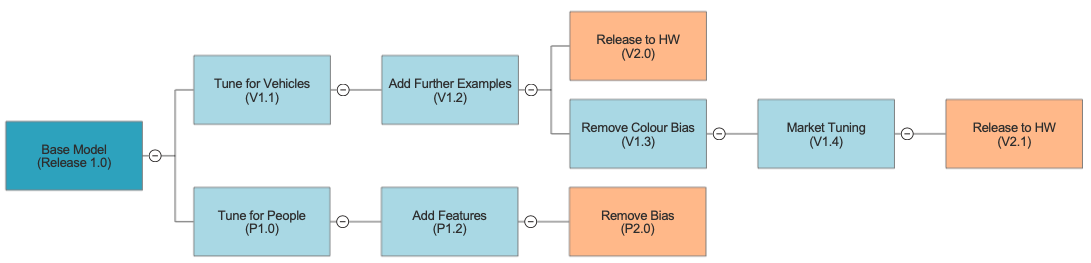
\includegraphics[width=2.5in]{lifecycle.png}
    \caption{Lifecycle of Models in Development Path}
    \label{fig_sim}
\end{figure}

To provide reference storage for the model repositories, we created two mongodb instances with the same collection structure. There are two collections - the signatures and the model data. This was to enable verification of the evolution path and when necessary pull the model synopsis for comparison.

\texttt{
    db.model.createIndex( {signature:1},{unique:true} )
    db.model.insertOne( { signature:'0x123412341234', creator:'brendanboner@gmail.com', previous:null, date:'01-01-2020 16:25' } )
}

\subsection{Comparing Models}
To ensure there is tracibility in between the models, if a parent model is defined, a \textit{b-score} is generated with a degree of difference between the models. The score is based on two factors, the difference between the model structure, and the difference between the two primary parameters for each layer: \textit{StdDev} \& \textit{Angle of Array}

\subsection{Collision Management}

{ \itshape
In computer science, a collision or clash is a situation that occurs when two distinct pieces of data have the same hash value, checksum, fingerprint, or cryptographic digest.[1]

Due to the possible applications of hash functions in data management and computer security (in particular, cryptographic hash functions), collision avoidance has become a fundamental topic in computer science.

Collisions are unavoidable whenever members of a very large set (such as all possible person names, or all possible computer files) are mapped to a relatively short bit string. This is merely an instance of the pigeonhole principle.[1]

The impact of collisions depends on the application. When hash functions and fingerprints are used to identify similar data, such as homologous DNA sequences or similar audio files, the functions are designed so as to maximize the probability of collision between distinct but similar data, using techniques like locality-sensitive hashing.[2] Checksums, on the other hand, are designed to minimize the probability of collisions between similar inputs, without regard for collisions between very different inputs.[3]
}


\subsection{Packaging}

the final area needed was determining how to distribute the mechanism for generatng and recording model representation artifacts. The solution was bundled together in a single package called \textit{lifecycle} that allows an existing solution to easily integrate the functions into the standard process. To demonstrate this, we bundled the lifecycle package into a single distributable wheel that was uploaded on a third party python notebook. As we were not able to guarantee that a local database was avaiable, we were able to setup a cloud instance of MongoDB on their Atlas platform that allowed us to run both local and central repositiories in the cloud. This was achieved by adding the following text to the start of the notebook/script:

\begin{lstlisting}[frame=single,basicstyle=\ttfamily]
from lifecycle import lifecycle_model
from lifecycle import lifecycle_db

mylifecycle = lifecycle_model()
mydb = lifecycle_db (
    username = '[db username]',
    password = '[password]',
    user='brendan.bonner2@mail.dcu.ie',
    organisation='Dublin City University',
    lifecycle=mylifecycle)

mydb.init_model_db()
\end{lstlisting}

